\subsection{Generic method}
\label{generic}

The generic branching method is a way more complex branching scheme but allows to keep subproblems with the knapsack structure. As the knapsack problem can be solved with dynamic programming, it allows to have a faster resolution method for the subproblems. However, several subproblems needs to be solved.

\subsubsection{Branching rules}

When a node is solved at optimality and that two branching items $i$ and $j$ have been found, we have to create one child where $w_{ij} \leq 0$ (the down branch) and one child where $w_{ij} \geq 1$ (up branch). For the down branch, we create a subproblem generating patterns with $x_i = 0$ and one subproblem generating patterns patterns with $x_i = 1, x_j=0$. Thus, the solution constructed includes patterns with items $i$ and $j$ separated. But in the solution, we only need one pattern with $x_i = 1, x_j=0$. The idea is to split the constraint $\sum_{p=1}^{P'} \alpha^p \leq B$ of \eqref{RMBPP} into the two following constraints :
\begin{equation}
	\label{generic-down}
	\left \{
	\begin{array}{l}
	\displaystyle \sum_{p \in \Pc' | x_i^p=1, x_j^p=0} \alpha^p \leq 1 \\
	\displaystyle \sum_{p \in \Pc' | x_i^p=0} \alpha^p \leq B-1 \\
	\end{array}
	\right.
\end{equation}
These two constraints preserves the number of patterns created but specify the number of patterns of each type. For the up branch, we create one subproblem generating patterns with $x_i = x_j = 0$ and one subproblem generating patterns patterns with $x_i = x_j = 1$. Thus, the solution is composed of patterns with $i$ and $j$ together and of (and patterns without $i$ and $j$). But we only need one pattern with $x_i = x_j = 1$ so we can split the constraint into the following new constraints :
\begin{equation}	
	\label{generic-up}
	\left \{
	\begin{array}{l}
	\displaystyle \sum_{p \in \Pc' | x_i^p= x_j^p=1} \alpha^p \leq 1 \\
	\displaystyle \sum_{p \in \Pc' | x_i^p= x_j^p=0} \alpha^p \leq B-1 \\
	\end{array}
	\right.
\end{equation}
These two constraints preserves the number of patterns created but specify the number of patterns of each type. For up and down branching rules, we can notice that the variables $x_i$ and $x_j$ are fixed so the subproblem keeps its knapsack structure if a preprocess is made. After fixing the branching variable, a knapsack problem remains to be solved (see \ref{generic_sp}).

The difficulty lies in the way to process several branches in a row. We have to introduce the notion of \textbf{branching set} which are composed of some \textbf{branching rules} (corresponding to the filter below the sum in \eqref{generic-down} and \eqref{generic-up}) and one \textbf{coefficient} (corresponding to the scalar 1 or $B-1$ in \eqref{generic-down} and \eqref{generic-up}). Each branching rule has several variables set to zero and several variables set to one. For example, 
\begin{equation*}
	\sum_{p \in \Pc' | \{x_1 = 0, x_2 = 1\} \cup \{x_3 = 0, x_4 = 1\}} \alpha^p \leq 1
\end{equation*}
is a branching set with branching rules $\{x_1 = 0, x_2 = 1\}$ and $\{x_3 = 0, x_4 = 1\}$ and with coefficient $1$ and 
\begin{equation*}
	\sum_{p \in \Pc' | \{x_1 = x_2 = 0\}} \alpha^p \leq B-1
\end{equation*}
is a branching set with branching rule $\{x_1 = x_2 = 0\}$ and with coefficient $B-1$. When a new node is created, we loop over all the branching sets of the parent node and create new sets for the child node by adding the new branching rules. From each parent branching set, at most two branching sets can be created for the child node. Four cases can happen : 

\begin{itemize}
	\item \textbf{The coefficient of the parent node branching set is L > 1} : \\
	In this case, the branching set have a unique rule by construction of the child nodes.
	\begin{itemize}
		\item \textbf{We have to add a down branching rule with items $i$ and $j$} : In this case, we create two branching sets for the child node. The two child branching sets are identical to the parent branching set with a little modification. In the first, the item $i$ is added to the variables set to 0 in the branching rules and the coefficient is set to $\L-\1$. In the second, the item $i$ is added to the variables set to 1 in the branching rules and the coefficient is set to $\1$.
	\end{itemize}
	\begin{itemize}
		\item \textbf{We have to add an up branching rule with items $i$ and $j$} : In this case, we create two branching sets for the child node. The two child branching sets are identical to the parent branching set with a little modification. In the first, the items $i$ and $j$ are added to the variables set to 0 in the branching rules and the coefficient is set to $\L-\1$. In the second, the items $i$ and $j$ are added to the variables set to 1 in the branching rules and the coefficient is set to $\1$.
	\end{itemize}
	\item \textbf{The coefficient of the parent node branching set is 1} : \\
	In this case, the branching set can have a multiple rule by construction of the child nodes. Only one of the patterns allowed to be created by the branching set can be used in the solution.
	\begin{itemize}
		\item \textbf{We have to add a down branching rule with items $i$ and $j$} : Only one set is created in the child node. For each branching rule in the parent node branching set, we add either $x_i = 0$ or $x_i=1, x_j=0$ to the child branching set containing the rules of the parent branching set. This new branching set has a coefficient equal to $\1$.
	\end{itemize}
	\begin{itemize}
		\item \textbf{We have to add an up branching rule with items $i$ and $j$} : Only one set is created in the child node. For each branching rule in the parent node branching set, we add either $x_i = x_j = 0$ or $x_i=x_j=1$ to the child branching set containing the rule of the parent branching set. This new branching set has a coefficient equal to $\1$.
	\end{itemize}
\end{itemize}

The way new constraints are added to the child nodes is a bit complicated as we have to handle multiple subproblems and we have to ensure that the coefficient of the branching sets add to $B$ in order to preserve the initial constraint $\sum_{p \in \Pc'} \alpha^p \leq B$ of \eqref{RMBPP} in each node. Of course, some of the rules created may be infeasible if one item is both in the set of variables set to 0 and 1. In this case, the rule is not included in the branching set. When the parent branching set is split into one feasible and one infeasible branching set, then we only keep the feasible branching set and the coefficient of the new set is equal to the coefficient of the parent branching set.
\begin{figure}[!ht]
	\centering
	\begin{minipage}{0.47\linewidth}
		\centering
		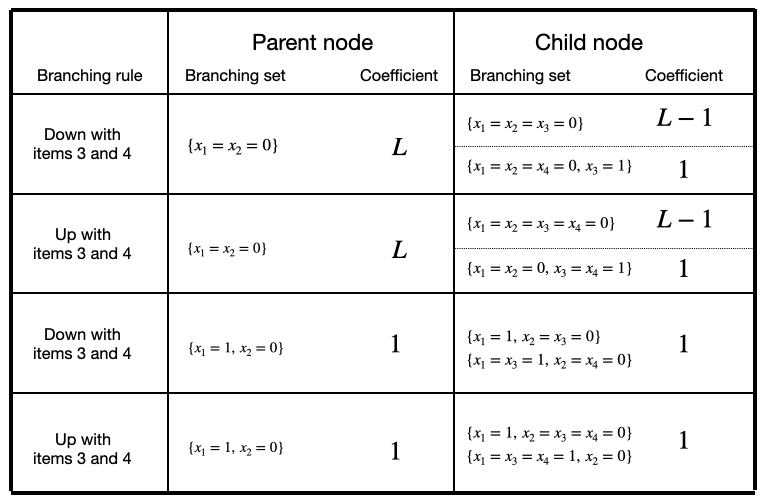
\includegraphics[width=0.7\linewidth]{img/generic-branching.png}
	\end{minipage}
	\begin{minipage}{0.47\linewidth}
		\centering
		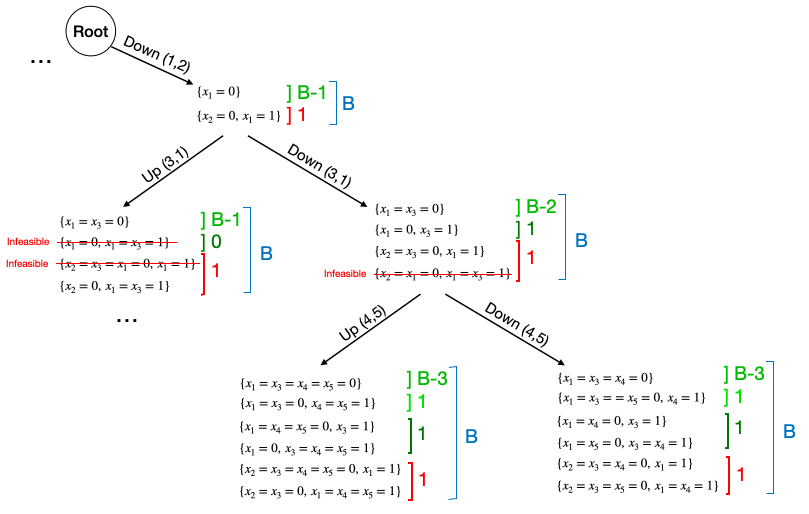
\includegraphics[width=\linewidth]{img/generic-example.png}
	\end{minipage}
	\caption{Left : The four cases presented above. Right : An example of how branching constraints are handled and how to proceed when a branching set is infeasible.}
\end{figure}

\subsubsection{Subproblem resolution}
\label{generic_sp}

In each node for the generic branching scheme, there are as many subproblems to solve as the total number of branching rules. Like for the Ryan \& Foster branching method, it is possible to use a LP solver like Gurobi. It can preprocess the problem by setting the variables to 0 or 1 according to the branching schemes before the solving process. But as the knapsack structure is preserved for each subproblem, it is possible to use dynamic programming instead of a classical solver which is usually slower. 

The first step before the dynamic programming process is to preprocess the data and treat the variables already fixed in the branching rules. For each variable set to 0, we simply remove this variable from the problem. For each variable set to 1, we remove the variable from the problem, decrease the knapsack capacity by the size of the item and add its cost to a preprocess cost. At the end of the preprocess, if the capacity of the knapsack is still positive, then the dynamic programming process can start. If the capacity is negative, then the knapsack problem is infeasible and the resolution is stopped here. At the end of the dynamic programming process, the total cost is the cost outputted by the dynamic program plus the preprocess cost. The items in the pattern are the items used in the dynamic program solution plus the items set to 1 during the preprocess step.

To solve dynamically the knapsack problem considering a capacity $C^{knap}$, items with sizes $s_i^{knap}$ and costs $p_i^{knap}$ for $i=1,\dots, I^{knap}$, we have to introduce $t_{i,c}^{knap}$, the maximal profit of a knapsack problem with capacity $c$ and with $i$ items in it among all the items. We can apply the following dynamic programming algorithm and backtracking method to find the optimal cost of the knapsack and the items involved in this optimal cost : 

\begin{figure}[!ht]
	\centering
	\begin{minipage}[t]{0.48\linewidth}
		\begin{algorithm}[H]
			\DontPrintSemicolon 
			\For{$i = 1,\dots, I^{knap}$}{
				\For{$c = 1,\dots,C^{knap}$}{
					\uIf{$s_i^{knap} > c$}{
						$t_{i+1,c} \leftarrow t_{i,c}$\;
					}\Else{
						$t_{i+1,c} \leftarrow \max \{t_{i,c} \ ; \  p_i^{knap} + t_{i,c-s_i^{knap}}\}$\;
					}
				}
			}
			\caption{Knapsack problem}
		\end{algorithm}
	\end{minipage}
	\hfill
	\begin{minipage}[t]{0.49\linewidth}
		\begin{algorithm}[H]
			\DontPrintSemicolon 
			Pattern $ \leftarrow \emptyset$\;
			$c = C^{knap}$\;
			\For{$i = I^{knap},\dots,1$}{
				\If{$t_{i,c} \neq t_{i-1,c}$}{
					Pattern $\leftarrow$ Pattern $\cup \ i$\;
					$c \leftarrow c -  s_i^{knap}$\;
				}
			}
			\caption{Knapsack problem, backtracking}
		\end{algorithm}
	\end{minipage}
\end{figure}
\newpage

\noindent The optimal cost is $t_{I^{knap}, C^{knap}}$ and the variable $Pattern$ contains the items involved in the optimal cost.

We can observe that the complexity of the dynamic program is $o(I^{knap}C^{knap})$. Although it can be way better than solving the subproblem using an IP solver, some issues can happen when the capacity of the knapsack is large. The dynamic program is not only size-dependant but also data-dependant in the way that two problems with the same number of items won't be solved in the same amount of time for different capacities. A problem with few items but with a huge capacity can be slower to solve than a problem with more items and a smaller capacity. In practice, it could be interesting to measure the solving time per number of items while using the solver and the solving time per number of items and capacity using dynamic programming in order to chose the solving method. Furthermore, as the dynamic programming method is implemented "by hand" in this project while the solver has been developed and optimized by a specialized team, the solver can still be faster in practice than the dynamic program even if the theoretical complexity is worst.